\documentclass[11pt, oneside]{article}   	% use "amsart" instead of "article" for AMSLaTeX format
\usepackage{geometry}                		% See geometry.pdf to learn the layout options. There are lots.
\geometry{letterpaper}                   		% ... or a4paper or a5paper or ... 
%\geometry{landscape}                		% Activate for rotated page geometry
\usepackage[parfill]{parskip}    		% Activate to begin paragraphs with an empty line rather than an indent
\usepackage{graphicx}				% Use pdf, png, jpg, or eps§ with pdflatex; use eps in DVI mode
								% TeX will automatically convert eps --> pdf in pdflatex		
\usepackage{amssymb}
\usepackage{amsmath}				% Math fonts
\usepackage{mathtools}				% Enable \coloneqq for := operator
\usepackage{hyperref}				% Enable links (especially for table of contents)
\hypersetup{						% Set link colors
    colorlinks,
    citecolor=black,
    filecolor=black,
    linkcolor=black,
    urlcolor=black
}
\geometry{top=8cm}

%SetFonts

%SetFonts

\renewcommand*\contentsname{Table of Contents}	% Change name of table of contents

\title{Gaussian Process Regression for Crowdfunding Campaigns Prediction}
\author{Victor Kristof}
\date{\today}								% Activate to display a given date or no date

\begin{document}
    \maketitle
    \newpage
    \newgeometry{margin=3cm}
    \tableofcontents
    \newpage
    \section{Introduction}
        \subsection{Notations}
        
            \begin{itemize}
                \item Let us denote $\mathbf{v}_{i:j}$, $i < j$ the subvector $\mathbf{u} = [v_i, ..., v_j]^T$ consisting of the elements $v_i$ to $v_j$ of the vector $\mathbf{v}$.
                %\item Let us denote $(v_{i:j}, i \leq j)$ the subsequence $(u_n, n = i, ..., j) = (v_i, ..., v_j)$ consisting of the elements $v_i$ to $v_j$ of the sequence $(v_n, n = 1, ..., N)$.
            \end{itemize}
        
   % \section{Gaussian Processes}
    \section{Problems Definition}
    
	\subsection{Single-Project Regression}
        
		\subsubsection*{Model}
             
                    We are first approaching the problem as time series regression, considering only one project. Our dataset $\mathcal{D} = \left\{ (x_i, y_i) \mid i = 1, ..., T \right\}$ consists of $T$ observations, with $x_i$ the time index corresponding to an amount of pledged money $y_i$. Hence, we have $X = [1, ..., T]^T$, a $(T \times 1)$ matrix of time indices, and $\mathbf{y} = [y_1, ..., y_T]^T$, a vector of observed values. We model the pledged money $f(X)$ at time indices $X$ as a Gaussian Process (GP):
                    
                    \begin{equation}
                    		f(X) \sim GP \left( m(X), k(X, X') \right). 
                    \end{equation}
                    
                    Our goal is to predict the future values of the pledged money $\mathbf{f}_{t:T} = f(X_{t:T})$ at future time indices $X_{t:T} = [t, ..., T]^T$ after observing the values $\mathbf{y}_{1:t} = [y_1, ..., y_t]^T$ at time indices $X_{1:t} = [1, ..., t]^T$. In the GP framework, we can compute this prediction using
                    
                    \begin{eqnarray}
            			\mathbf{f}_{t:T}  \mid X_{1:t}, \mathbf{y}_{1:t}, X_{t:T} 	& \sim & 	\mathcal{N}\left(\overline{\mathbf{f}}_{t:T}, \text{ cov}(\mathbf{f}_{t:T})  \right) \\ 
           			\overline{\mathbf{f}}_{t:T}							& = & 	K(X_{t:T}, X_{1:t}) \left[ K_{1:t} + \sigma_n^2I \right]^{-1}\mathbf{y}_{1:t} \label{eq:predictive_mean} \\
           			\text{cov}(\mathbf{f}_{t:T}) 						& = & 	K_{t:T} - K(X_{t:T}, X_{1:t})\left[ K_{1:t} + \sigma_n^2I \right]^{-1}K(X_{1:t}, X_{t:T}) \label{eq:predictive_variance},
                    \end{eqnarray}
                    
                    with $K_{1:t} \coloneqq K(X_{1:t}, X_{1:t})$ and $K_{t:T} \coloneqq K(X_{t:T}, X_{t:T})$. Finally, the model's optimal hyperparameters $\theta_*$ are learned by maximizing the \textit{log marginal likehood} over the first $t$ observed values:
                    
                    \begin{eqnarray}
                    		\theta_* 	&=& \underset{\theta} {\arg\max} \log p(\mathbf{y_{1:t}} \mid X_{1:t}, \theta) \\
    						&=& \underset{\theta} {\arg\max} \left\{ -\frac{1}{2}\mathbf{y}_{1:t}^T \left[ K_{1:t}+ \sigma_n^2I \right]^{-1}\mathbf{y}_{1:t} -\frac{1}{2}\log det\left[K_{1:t}+ \sigma_n^2I\right] -\frac{t}{2}\log 2\pi \right\} \label{eq:arg_max_log_marginal_likelihood}.
                    \end{eqnarray}
                                                   
		\subsubsection*{Results}
            		The major problem in this context was that the predictive mean $\mathbf{f}_*$ always falls back to the mean $m(\mathbf{x})$ very quickly. One solution is to sum two squared-exponential kernels and initializing one of them to a large length-scale in order to capture the global trend. This yields to some reasonable results. However, when using a model trained on one project to predict the future values of another one gives very poor performances.
           
         \subsection{Multi-Project Regression}
         	\subsubsection*{Model}
        			Our next idea is to consider $P$ projects and try to learn the hyperparameters $\theta$ over various time series at the same time. In this case, for a given project $p$, we have a dataset $\mathcal{D}^{(p)} = \left\{ (x_i^{(p)}, y_i^{(p)}) \mid i = 1, ..., T \right\}$. Again, $y_i^{(p)}$ is the amount of pledged money at each time index $x_i^{(p)}$. Note that we have $x_i^{(p)}= x_i = i$, for all $p=1,...,P$ and all $i=1,...,T$. We combine the projects together to obtain the full dataset $\mathcal{D} = \left\{ \mathcal{D}^{(p)} \mid p = 1, ..., P \right\}$ (\textit{multi-task learning}). We then have the input $X = [1, ..., T]^T$, a $(T \times 1)$ matrix of time indices, and the output $Y = \left[\mathbf{y}^{(p)} \right]_{p=1}^P$, a $(T \times P)$ matrix of observed values per project. For a given project $p$, we are trying to predict the pledged money $\mathbf{f}_{t:T}^{(p)} = f(X_{t:T}^{(p)})$ at future time indices $X_{t:T}^{(p)} = [t,...,T]^T$ after observing the values $\mathbf{y}_{1:t}^{(p)}$ at time indices $X_{1:t}^{(p)} = [1, ..., t]^T$. To do so in the GP framework, we have
        
                        \begin{equation}
                        		\mathbf{f}_{t:T}^{(p)} \mid X_{1:t}^{(p)}, \mathbf{y}_{1:t}^{(p)}, X_{t:T}^{(p)} \sim \mathcal{N} \left( \overline{\mathbf{f}}_{t:T}^{(p)}, \text{ cov}(\mathbf{f}_{t:T}^{(p)}) \right),
                		\end{equation}
                		        
                        with $\overline{\mathbf{f}}_{t:T}^{(p)}  $ and $\text{cov}(\mathbf{f}_{t:T}^{(p)}) $ obtained similarly to Equations \ref{eq:predictive_mean} and \ref{eq:predictive_variance}. The model's optimal hyperparameters $\theta_*$ are learned similarly to Equation \ref{eq:arg_max_log_marginal_likelihood} by maximizing the log marginal likelihood over all the projects, that is
                        
                        \begin{equation}
                        		\theta_* = \underset{\theta} {\arg\max} \sum_{p=1}^P \log p(\mathbf{y}^{(p)} \mid X^{(p)}, \theta).
                        \end{equation}
                        
                        Note that in this case, we consider the ``full" projects, that is $\mathbf{y}^{(p)} = \mathbf{y}_{1:T}^{(p)}$ and $X^{(p)} = X_{1:T}^{(p)}$.
                        
         	\subsubsection*{Results}
        			Again, we couldn't obtain good results with this approach, as the predictions always fall back very quickly to the mean of the GP. [MORE DETAILS]
        
         \subsection{Project Classification}
         	\subsubsection*{Model}
            		We then decide to perform a simpler task. Instead of trying to predict future amounts of pledged money after some observations, we try now to classify whether a project $p$ will be successful ($c^{(p)} = 1$) or not ($c^{(p)} = 0$). Indeed, by separating the dataset in two classes (\textit{successful} and \textit{failed}), we notice that they have a very different profiles, as shown in Figure \ref{fig:two_profiles}, and therefore should be easy to discriminate. To do so, we train one GP using the successful projects and one using the failed projects. We then try to determine whether a new, partially observed project will be successful or not. 
			\begin{figure}[h]
                        		\begin{center}
                        			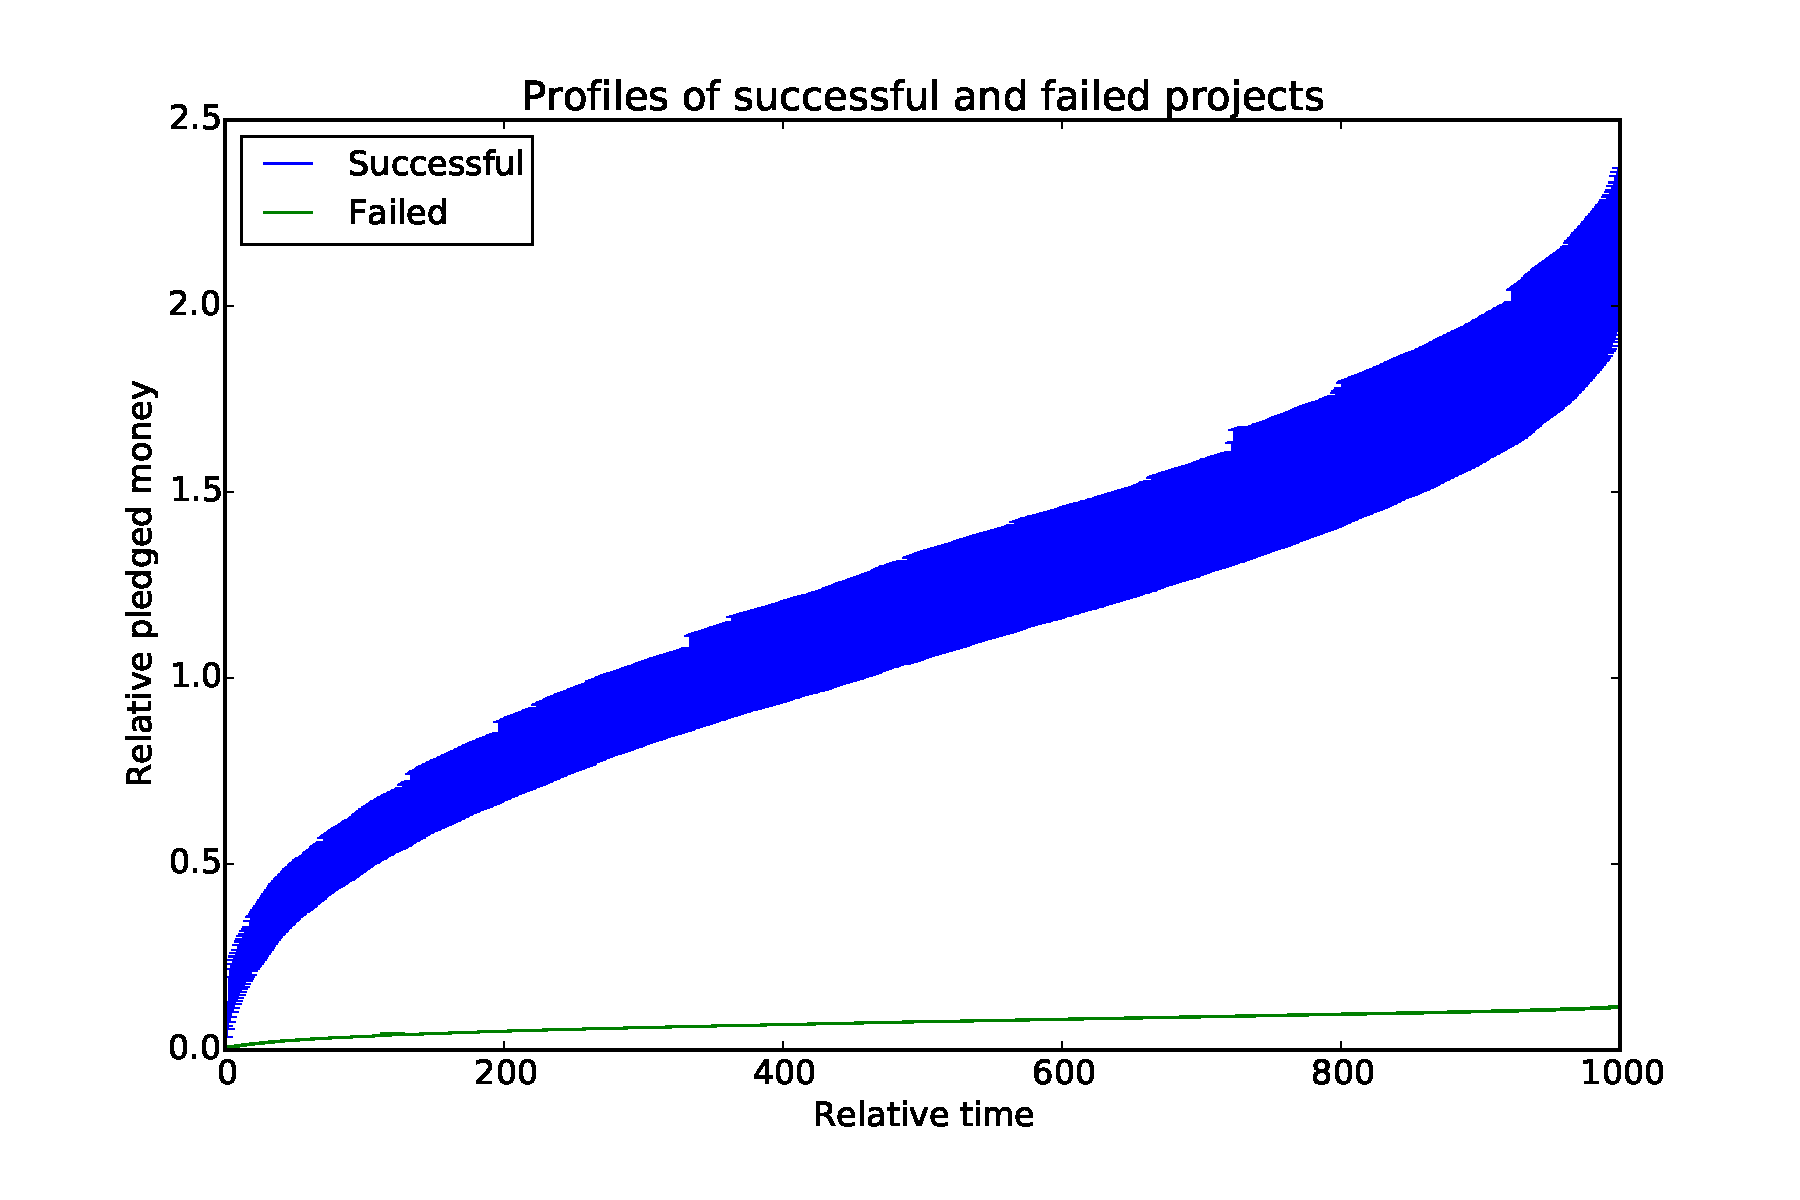
\includegraphics[scale=0.5]{img/two_profiles.pdf}
                        			\caption{Average and normalized standard deviation for both classes displaying two very distinct profiles that suppose the possibility to classify the projects.}
                       		 	\label{fig:two_profiles}
                       	 	\end{center}
                        	\end{figure}
			We learn $\theta_s$ the hyperparameters of a GP over $P_s$ successful projects  and $\theta_f$ the hyperparameters of a GP over the $P_f$ failed projects. That is, we obtain th''e two sets of hyperparameters by maximizing the log marginal likelihoods
        
                        \[\theta_s = \underset{\theta} {\arg\max} \sum_{p=1}^{P_s} \log p(\mathbf{y}_s^{(p)} \mid X^{(p)}, \theta)\]
                        \[\theta_f = \underset{\theta} {\arg\max} \sum_{p=1}^{P_f} \log p(\mathbf{y}_f^{(p)} \mid X^{(p)}, \theta),\]
                        
                        where $\mathbf{y}_s$ and $\mathbf{y}_f$ denote the observations of the successful and failed projects respectively. We then determine the success state $c^{(p)}$ of a new project $p$ with partial observations $\mathbf{y}_{1:t}^{(p)}$ as
                        
                        \[c^{(p)} = 
                        \begin{cases}
                            1, & \text{ if } \log p(\mathbf{y}_{1:t}^{(p)} \mid X_{1:t}, \theta_s) > \log p(\mathbf{y}_{1:t}^{(p)} \mid X_{1:t}, \theta_f) \\
                            0, & \text{ otherwise }
                        \end{cases}.\]
            
         	\subsubsection*{Results}
		[TO BE COMPLETED]
        
         \subsection{Output as Input}
         	\subsubsection*{Model}
        			We change completely the set up. Instead now of using the time as input and trying to predict the pledged money at new time indices, we now consider the pledged money at each time step as input and the last time index as the output. That is, we have now a dataset $\mathcal{D} = \left\{ (\mathbf{x}^{(p)}, y^{(p)}) \mid p = 1, ..., P \right\}$ with $\mathbf{x}^{(p)} = \mathbf{y}_{1:t}^{(p)}$ and $\mathbf{y}^{(p)} = y_T^{(p)}$. We then have $X = \left[\mathbf{x}^{(p)}\right]_{p=1}^P$, a $(P \times t)$ matrix of pledged money, and $\mathbf{y} = \left[y_T^{(p)}\right]_{p=1}^P$, a $(P \times 1)$ vector corresponding to the total amount of money at the end of the campaign. The difference with the previous approach is that now the features for each project are the amount of pledged money at different time steps and not the same (shared) input values $[1,...,T]^T$. Note that $t$ can be arbitrarily set to any value up to $T-1$ and that the number of samples taken in $[1, t]$ can also be determined arbitrarily.
        
        			Our goal now is to predict, for a new project $p$, the final amount of pledged money $y_T^{(p)} = f(\mathbf{y}_{1:t}^{(p)})$ given $\mathbf{y}_{1:t}^{(p)}$ the money received up to time $t$ after observing the total pledged money for all projects $\mathbf{y} = \left[y_T^{(p)}\right]_{p=1}^P$ and the money they received up to time $t$, $X = \left[ \mathbf{y}_{1:t}^{(p)} \right]_{p=1}^P$. In the GP framework, we can compute this prediction using
        			 
			 \begin{eqnarray}
			 	y_T^{(p)} \mid X, \mathbf{y}, \mathbf{y}_{1:t}^{(p)} 	& \sim & 	\mathcal{N}\left(\overline{y}_T^{(p)}, \text{ cov}(y_T^{(p)})  \right) \\
                            	\overline{y}_T^{(p)}							& = &	K(\mathbf{y}_{1:t}^{(p)}, X) \left[ K(X, X) + \sigma_n^2I \right]^{-1}\mathbf{y} \\
                            	 \text{cov}(y_T^{(p)}) 						& = & 	K(\mathbf{y}_{1:t}^{(p)}, \mathbf{y}_{1:t}^{(p)}) - K(\mathbf{y}_{1:t}^{(p)}, X)\left[ K(X, X) + \sigma_n^2I \right]^{-1}K(X, \mathbf{y}_{1:t}^{(p)}).
                            \end{eqnarray}

                                   
        			As seen in Figure \ref{fig:input_output_global}, it seems impossible to do a regression considering all the projects together. However, the two modes corresponding to the successful and failed projects are clearly distinguisable. Therefore we try to perform the regression on each of the two classes separately. 
			
			\begin{figure}[h]
                        		\begin{center}
                        			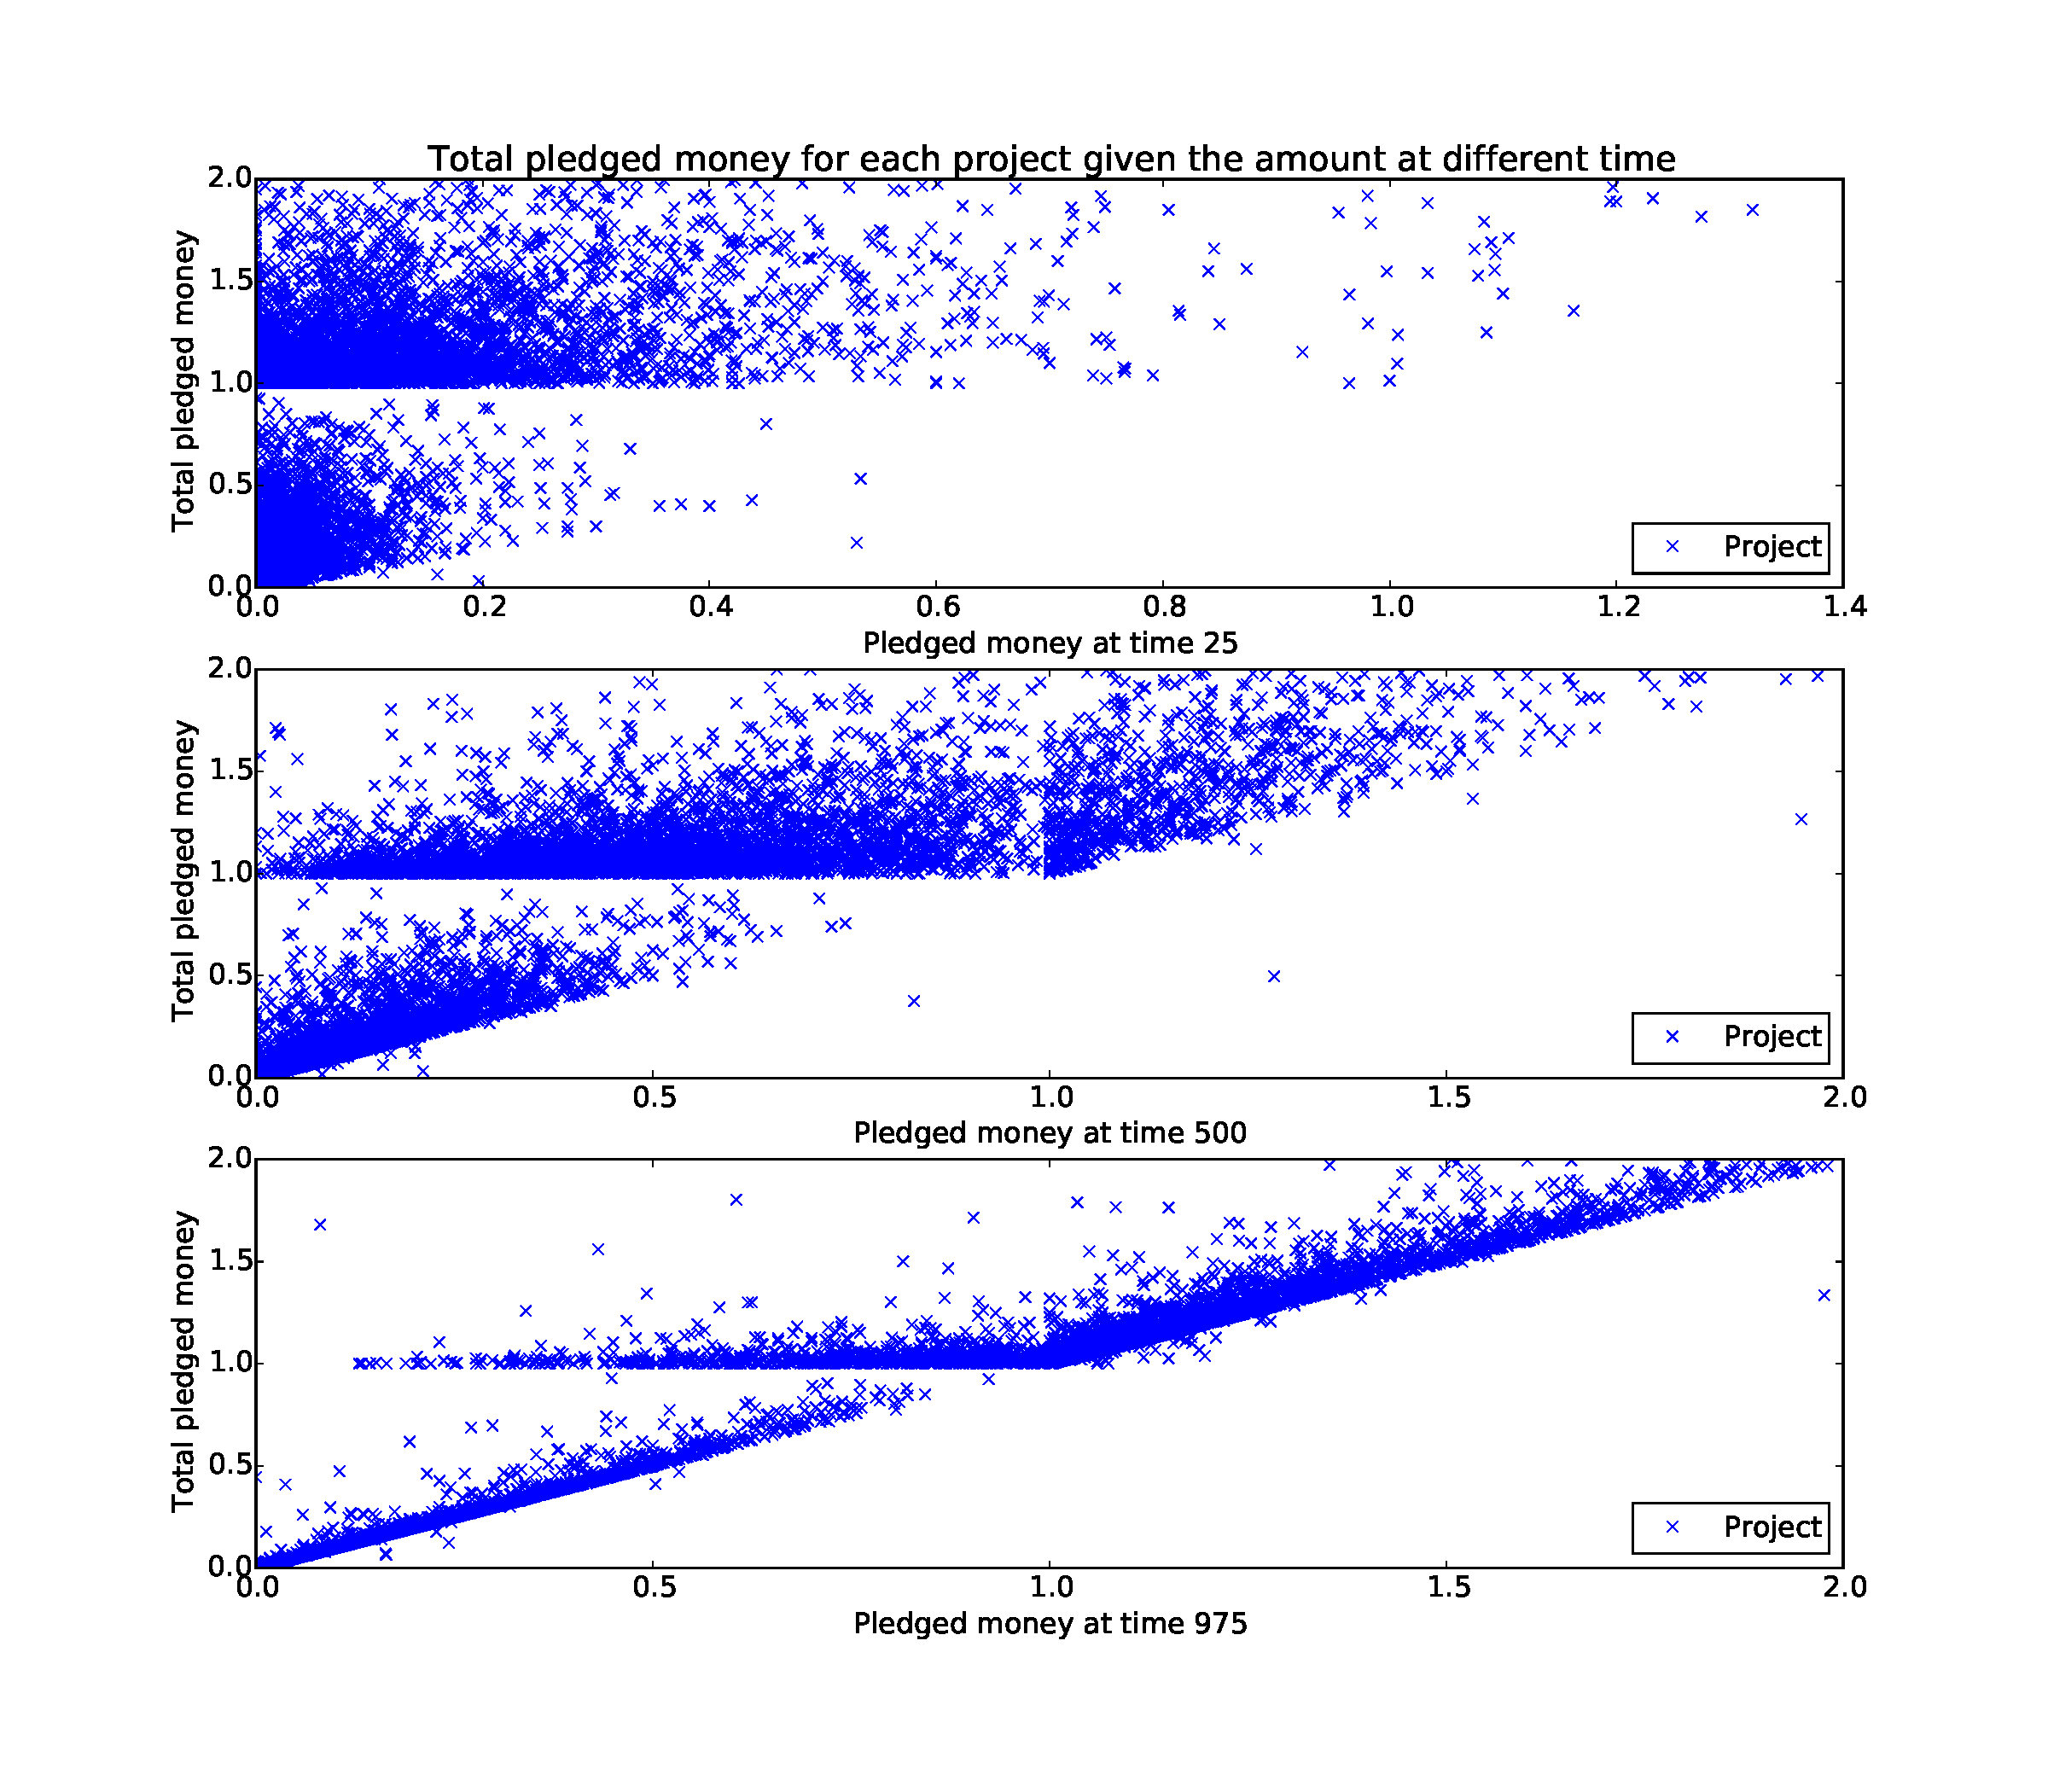
\includegraphics[scale=0.5]{img/input_output_global}
                        			\caption{Total pledged money for each project versus the amount they had at time 10.}
                       		 	\label{fig:input_output_global}
                       	 	\end{center}
                        	\end{figure}
        
        		\subsubsection*{Results}
        			[TO BE COMPLETED] Mixture of models can probably be used as other (latent) modes may exist.
        
         \subsection{Mixture of Gaussian Processes}
         	\subsubsection*{Model}
        		\subsubsection*{Results}
		
         \subsection{Mixture of Least Squares}
         	\subsubsection*{Model}
        		\subsubsection*{Results}    
    
\end{document}  